\documentclass{sigchi-ext}
% Please be sure that you have the dependencies (i.e., additional
% LaTeX packages) to compile this example.
\usepackage[T1]{fontenc}
\usepackage{textcomp}
\usepackage[scaled=.92]{helvet} % for proper fonts
\usepackage{graphicx} % for EPS use the graphics package instead
\usepackage{balance}  % for useful for balancing the last columns
\usepackage{booktabs} % for pretty table rules
\usepackage{ccicons}  % for Creative Commons citation icons
\usepackage{ragged2e} % for tighter hyphenation

% Some optional stuff you might like/need.
% \usepackage{marginnote} 
% \usepackage[shortlabels]{enumitem}
% \usepackage{paralist}
% \usepackage[utf8]{inputenc} % for a UTF8 editor only

%% EXAMPLE BEGIN -- HOW TO OVERRIDE THE DEFAULT COPYRIGHT STRIP --
% \copyrightinfo{Permission to make digital or hard copies of all or
% part of this work for personal or classroom use is granted without
% fee provided that copies are not made or distributed for profit or
% commercial advantage and that copies bear this notice and the full
% citation on the first page. Copyrights for components of this work
% owned by others than ACM must be honored. Abstracting with credit is
% permitted. To copy otherwise, or republish, to post on servers or to
% redistribute to lists, requires prior specific permission and/or a
% fee. Request permissions from permissions@acm.org.\\
% {\emph{CHI'14}}, April 26--May 1, 2014, Toronto, Canada. \\
% Copyright \copyright~2014 ACM ISBN/14/04...\$15.00. \\
% DOI string from ACM form confirmation}
%% EXAMPLE END

% Paper metadata (use plain text, for PDF inclusion and later
% re-using, if desired).  Use \emtpyauthor when submitting for review
% so you remain anonymous.
\def\plaintitle{Shared Story: Constructing Identity and Local Community through Tangible Exploration} \def\plainauthor{Diego Salvatierra, Po Tsui}
\def\emptyauthor{}
\def\plainkeywords{Identity construction environment; child-computer interaction; youth; education; tangible user interfaces}
\def\plaingeneralterms{Documentation, Standardization}

\title{Shared Story: Constructing Identity and Local Community through Tangible Exploration}

\numberofauthors{2}
% Notice how author names are alternately typesetted to appear ordered
% in 2-column format; i.e., the first 4 autors on the first column and
% the other 4 auhors on the second column. Actually, it's up to you to
% strictly adhere to this author notation.
\author{%
  \alignauthor{%
    \textbf{Diego Salvatierra}\\
    \affaddr{Stanford University} \\
    \affaddr{Stanford, CA 94305, USA} \\
    \email{dsalva@stanford.edu} }\alignauthor{%
    \textbf{Po Tsui}\\
    \affaddr{Stanford University}\\
    \affaddr{Stanford, CA 94305, USA}\\
    \email{potsui@stanford.edu} } }

% Make sure hyperref comes last of your loaded packages, to give it a
% fighting chance of not being over-written, since its job is to
% redefine many LaTeX commands.
\definecolor{linkColor}{RGB}{6,125,233}
\hypersetup{%
  pdftitle={\plaintitle},
%  pdfauthor={\plainauthor},
  pdfauthor={\emptyauthor},
  pdfkeywords={\plainkeywords},
  bookmarksnumbered,
  pdfstartview={FitH},
  colorlinks,
  citecolor=black,
  filecolor=black,
  linkcolor=black,
  urlcolor=linkColor,
  breaklinks=true,
}

% \reversemarginpar%

\begin{document}

%% For the camera ready, use the commands provided by the ACM in the Permission Release Form.
%\CopyrightYear{2007}
%\setcopyright{rightsretained}
%\conferenceinfo{WOODSTOCK}{'97 El Paso, Texas USA}
%\isbn{0-12345-67-8/90/01}
%\doi{http://dx.doi.org/10.1145/2858036.2858119}
%% Then override the default copyright message with the \acmcopyright command.
%\copyrightinfo{\acmcopyright}

\maketitle

% Uncomment to disable hyphenation (not recommended)
% https://twitter.com/anjirokhan/status/546046683331973120
\RaggedRight{} 

% Do not change the page size or page settings.
\begin{abstract}
Students in highly segregated communities rarely have a chance to share their life stories with people from other backgrounds. They may also be unaware of how their life story has been shaped by their community history. Shared Story aims to help middle and high school students reflect on their life stories and share these stories with others in their community, via a map and timeline on a tangible user interface (TUI) table, where individuals construct physical and digital representations of important events in their lives and their communities. They can also then share their stories and explore others online via an integrated web application. By viewing the events placed by themselves and others, young learners will become aware of how others in their community lead their lives and what places and events have shaped them.
\end{abstract}

\keywords{\plainkeywords}

\category{H.5.m}{Information interfaces and presentation (e.g.,
  HCI)}{Miscellaneous}\category{See}{\url{http://acm.org/about/class/1998/}}{for
  full list of ACM classifiers. This section is required.}

\section{Introduction}
In today's classrooms, too little time is spent on reflection of personal history (Darder). There also exist a general lack of knowledge of community history, which in turns exacerbates the division caused by urban segregation. We are motivated to address these issues by proposing a design that would enanable middle and high school students to construct and share their life stories and explore how their community's history connects with these stories.

\section{Theoretical Framework}
We draw as inspiration Freire's argument that learners should become aware of their world, its social and political conditions, and their position within it. Through the lens of critical pedagogy, our project aims to help learners engage in the "constant unveiling of reality" that is their surrounding community and personal histories. By allowing learners to construct personally significant places and events on a physical timeline and map, we help students undertake the process of creating and changing their reality.

We also draw on Erikson's work on the "identity vs. role confusion stage" experienced by adolescents, during which they seek historical frameworks, identities, and roles in which to make sense of who they are. Through our project, we aim to help them understand the events that "determine others" and themselves.

\begin{marginfigure}[-25pc]
  \begin{minipage}{\marginparwidth}
    \centering
    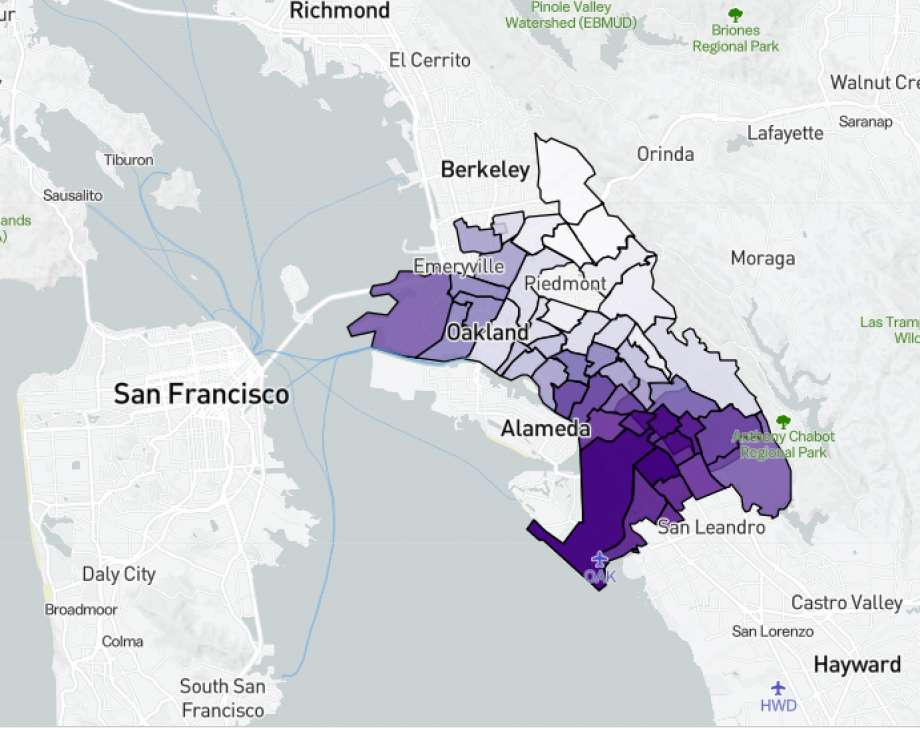
\includegraphics[width=0.9\marginparwidth]{figures/map}
    \caption{School segregation in the Bay Area. Source: Vox, \textit{We can draw school zones to make classrooms less segregated. This is how well your district does.} 2018.}~\label{fig:bay-area-map}
  \end{minipage}
\end{marginfigure}

Additionally, we consider the high segregation in schools by race and class within the United States (Fig. 1), and follow the spirit of Lopez and Nastasi's work which brought together youth from suburban and urban school districts and resulted in increased "democratic participation." Our project mirrors their pedagogical components of helping students understand their own identities and those of their peers.

\section{Technological Framework}
Learners engage with our learning goals through what Papert calls an "object-to-think-with," which help learners grasp certain abstract concepts through tangible means and share ideas with the world. Our project builds on his constructionist framework by allowing learners to create physical representations of their memories and perceptions of their surroundings. 

Drawing on Horn's work, our use of a TUI table evokes the cultural form of the table top around socialization and play through a more familiar and child- (rather than parent-) driven design. Additionally, the work of Petrelli, Whittaker, and Brockmeier on mementos and autotopographies indicate that physical mementos play a large role in triggering memories, and suggest potential in augmenting objects with digital memories. In our design, physical 3D-printed representations of events and places are augmented with digital (textual and symbolic) representations. In such a way we allow students to engage in the critical "meaning construction" stemming from their personal memories.

Finally, we introduce a shared screen with aggregated stories overlaid together on a single map as a way to create a multi-user environment which encourages community building and lends the user a social context in which to construct their personal history. The collaborative maps become an object for students to reflect upon their lives and their communities, and to share them publicly with the world.

\section{Related Work}

Our project aligns with Bers's work on Identity Construction Environments (ICE), which are "technological tools purposefully designed to afford opportunities for exploring identity and engaging in reflection and discussion about personal and moral values." We abide by the five principles she puts forth, which involve purposeful design to help young people learn about and construct their identity through community, storytelling, and dynamic objects representing the self.

We study Zora, a multi-user virtual environment that allows learners to design and participate within a graphical virtual city and its social organization. While Zora is situated within a virtual world and thus one level removed from the physical community in which the student lives, we in contrast use the actual neighborhood as touchpoints for reflection and transforming action. We ground our users to their immediate surroundings and aim in Freirean fashion to lead to direct action upon the learner's world. Students learn about the actual history of their immediate surrounding community and the lives of their peers. We thus also differ from Zora's approach by placing an emphasis on the historicity of the individual and the community. We aim for learners to make sense of their own lived experiences and recognize themselves in the context of their community and family history. Finally, the design allows for users to view their construction as one whole, through which macro-level insights can emerge.

\section{Design}
Shared Story is a collection of collaborative maps and timeline on a tangible user interface (TUI). We intend the table to be located in a public shared space, such as a museum or public library, such that middle and high school students can regularly pass through and contribute their personal constructions. Students engage in personal reflection which acknowledges their own historicity and dynamic self, engage in their local community and its history, and develop peer empathy through exploration of shared stories.


\begin{marginfigure}[-57pc]
  \begin{minipage}{\marginparwidth}
    \centering
    \includegraphics[width=0.9\marginparwidth]{figures/web}
    \caption{Web view: aggragated stories on a shared map}~\label{fig:web}
  \end{minipage}
\end{marginfigure}

\begin{marginfigure}[-36pc]
  \begin{minipage}{\marginparwidth}
    \centering
    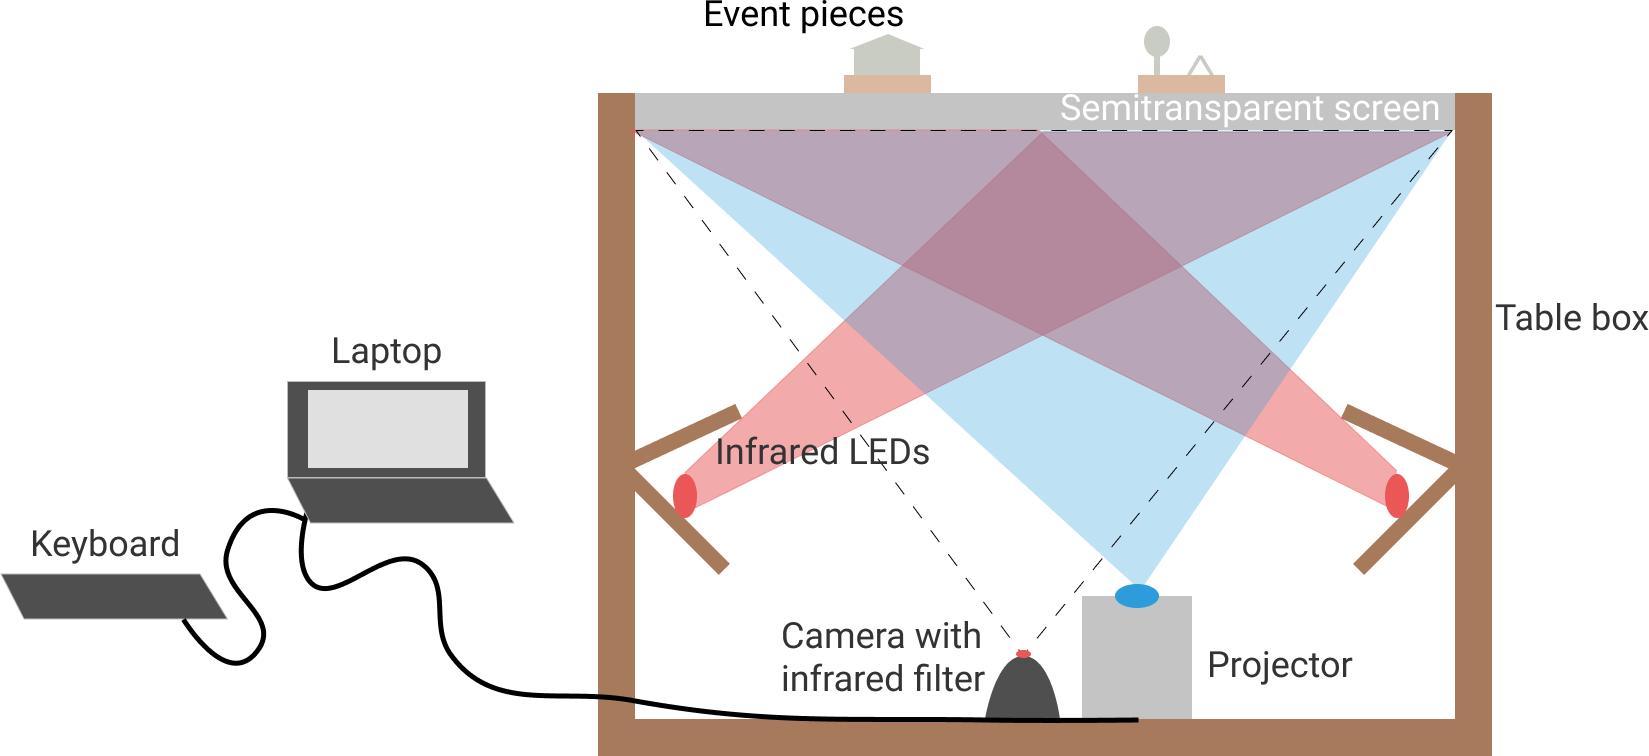
\includegraphics[width=0.9\marginparwidth]{figures/tui}
    \caption{Our tangible user interface table design}~\label{fig:tui}
  \end{minipage}
\end{marginfigure}

\begin{marginfigure}[-14pc]
  \begin{minipage}{\marginparwidth}
    \centering
    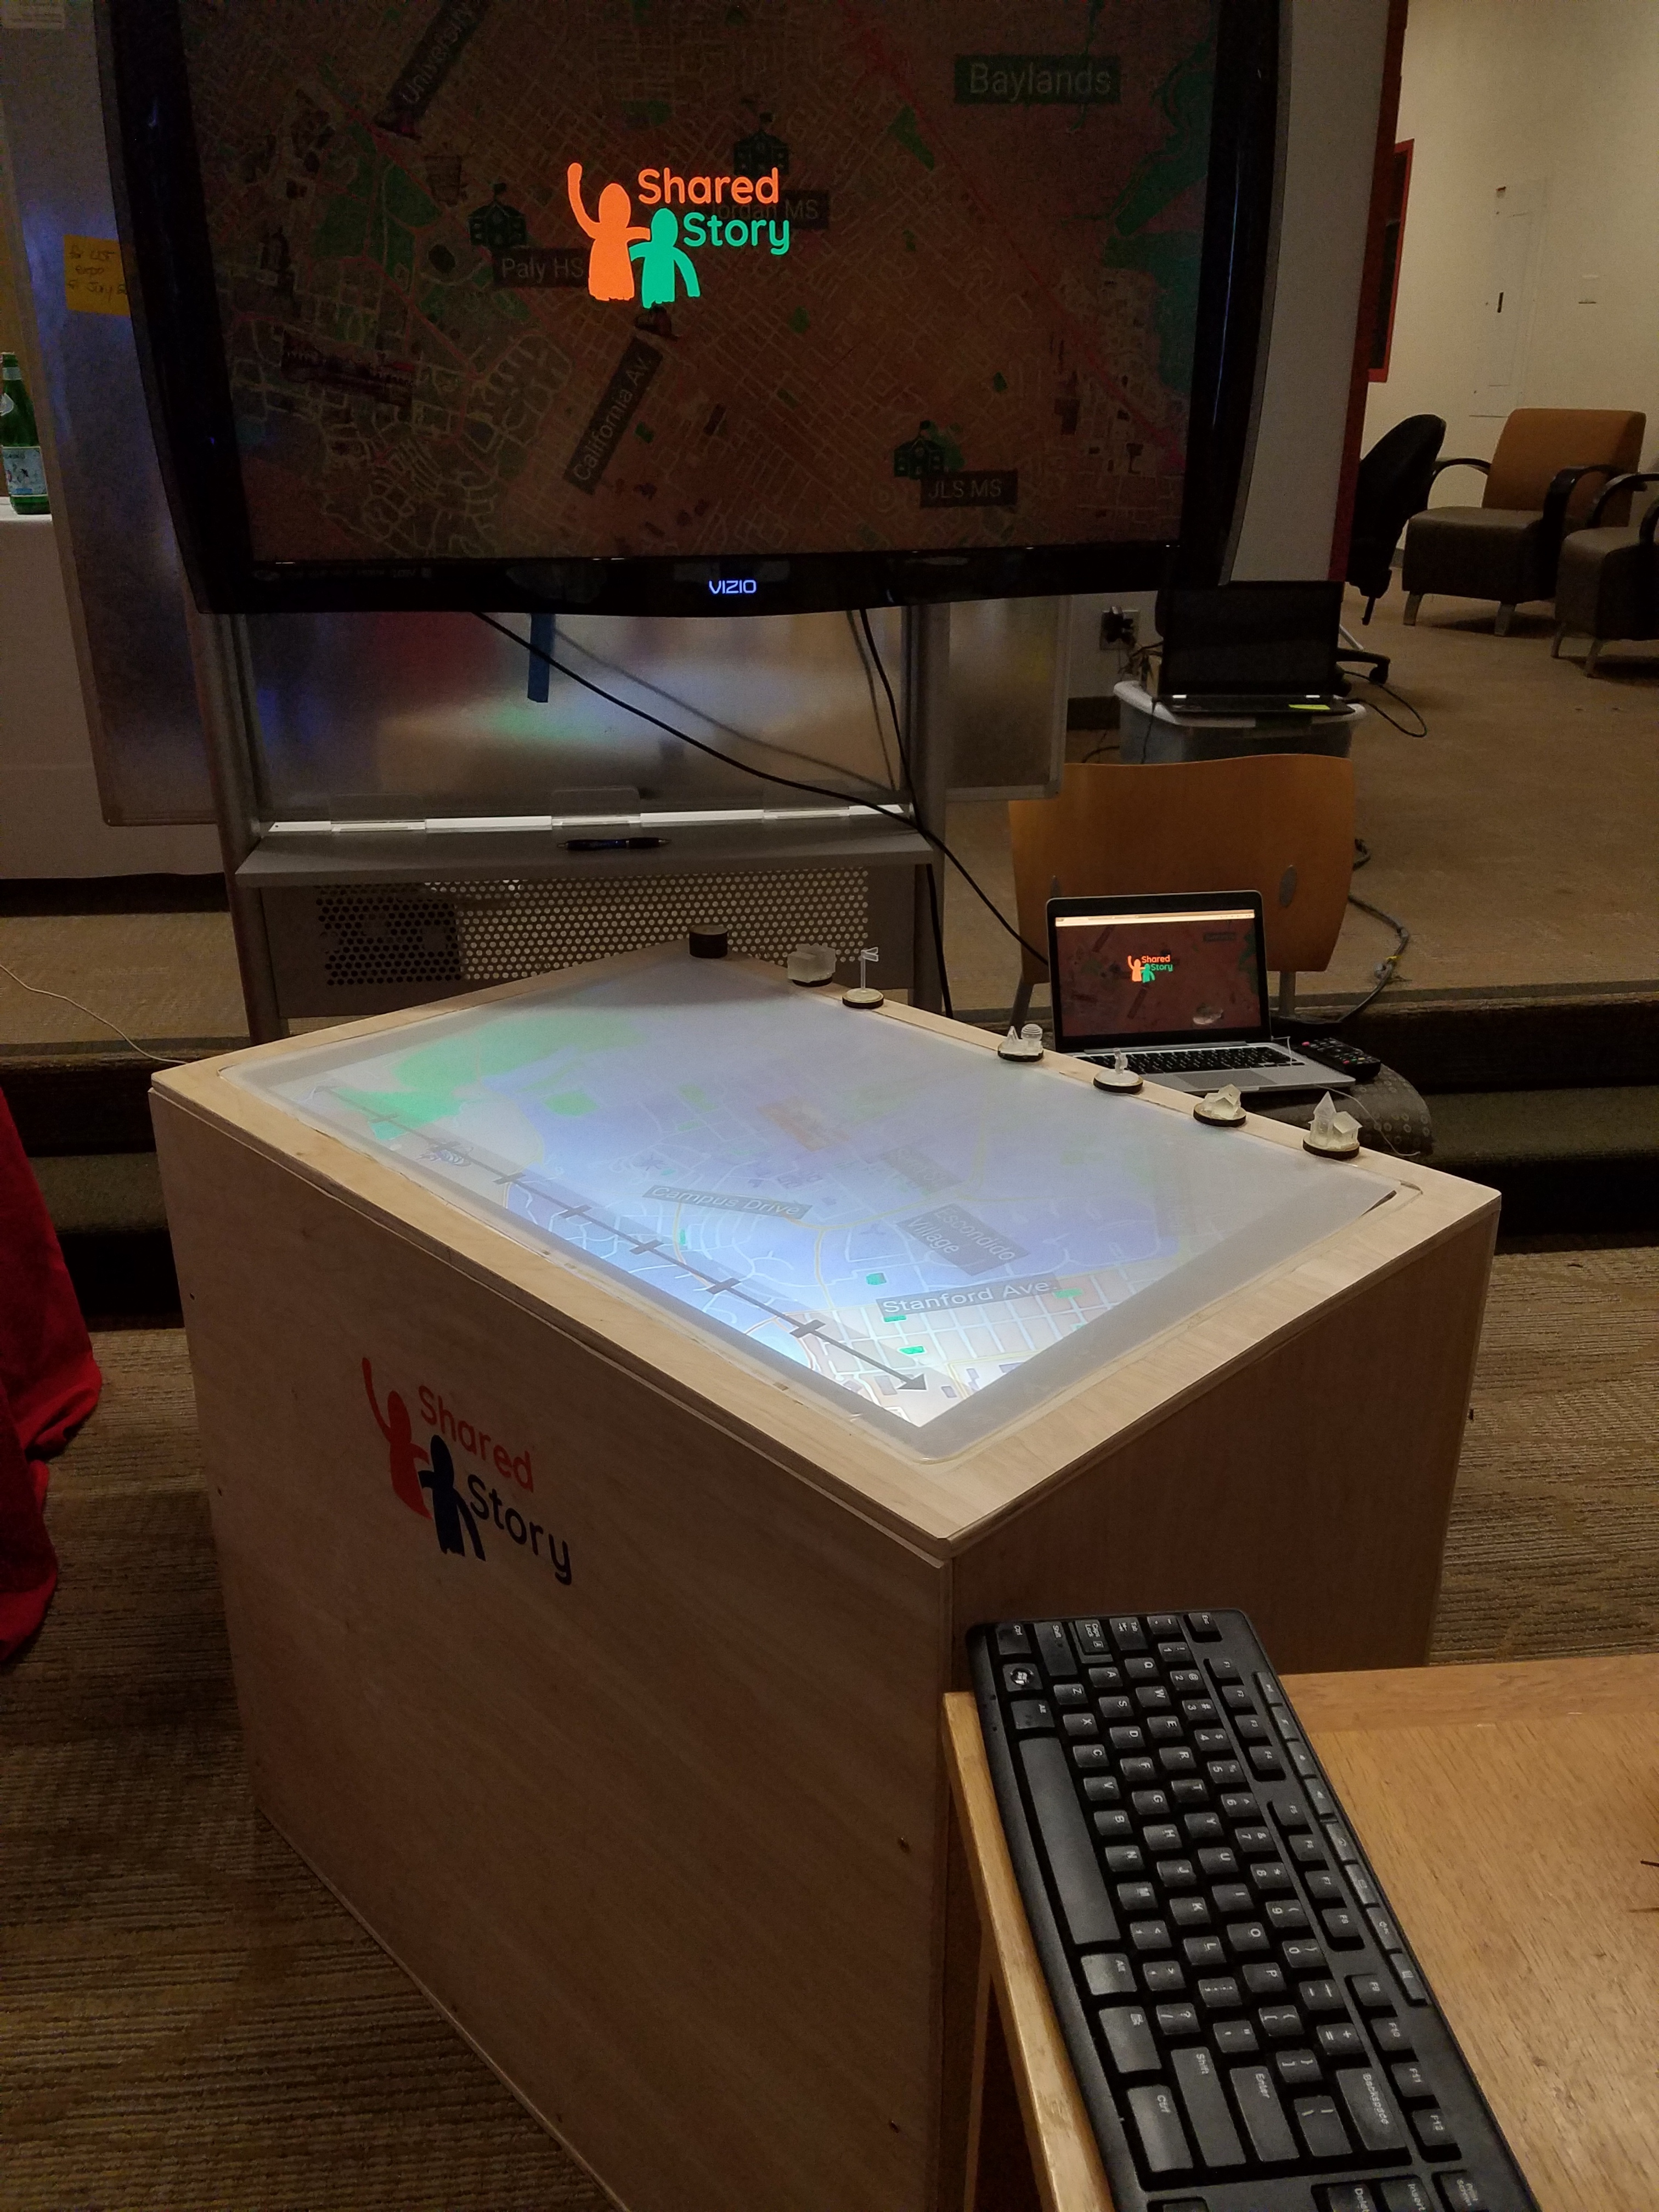
\includegraphics[width=0.9\marginparwidth]{figures/table}
    \caption{The Shared Story table and web view}~\label{fig:table}
  \end{minipage}
\end{marginfigure}


Our project allow learners the following actions:

\begin{enumerate}\compresslist
	\item \textbf{Choosing your map} Students first choose a map representing their local community. To encourage playful exploration, we designed each map with a watercolor-styled base layer (from \url{http://maps.stamen.com/watercolor}) and label with major streets, schools, and landmarks for students to easily orient themselves. Students choose a map by placing a marker on the table top's screen.

	\item \textbf{Placing events on the map} Students then place physical event markers, with a corresponding digital icon, on the screen. We currently support the following icons: home, school, religion, outdoors, social movement, and street/other.

	\item \textbf{Adding events to timeline} Similarly, students can also add events to a timeline at the bottom of each map to interact with events on a time dimension.

	\item \textbf{Adding event descriptions} Once an icon has been placed, learners can type an accompanying description using a keyboard connected to the table.

	\item \textbf{Saving and sharing the map} Students can save their constructed maps by placing a wooden icon labeled "save" on the screen, which freezes the screen and uploads the events to an online database. The aggregated events across all students within a community can be viewed online on a single map (Fig. 2).
\end{enumerate}

\section{Technical Construction}

Our TUI table (Fig. 3 and 4) is inspired by the design put forth by Konrad and Jung and existing tables at the Transformative Learning Technologies Lab (TLTL) at Stanford University. We modify the design by connecting a keyboard for learners to input their event description. We also constructed a wood-paneled box for the table, which helps maintain a controlled lighting environment.

We use the ReactiVision library to recognize fiducial patterns on the bottom of the physical event markers; this is then streamed as input to our Processing application that runs the graphics on the TUI table. The data is stored in a Firebase database and is viewable as a shared map at \url{sharedstory.herokuapp.com}, a Node.js server we built and hosted on Heroku.

\section{Future Work}
Our next step is to conduct user testing in a public space. In the future, we hope to enable learners to upload photos and artwork per event as an additional level of personalization and self-expression. We also see significant potential in manipulating the aggregated events to identify macro-level patterns and incorporate a more explicit social justice lens that visualizes issues such as urban segregation.

\section{Conclusion}
We propose Shared Story as a social tangible interface design project that allows middle and high school students to reflect on and share their life stories with others in their community. We build on constructionist principles, emphasize Freire's focus on conscientization and Erikson's theories of identity formation, and learn from prior work such as Zora. Users place physical objects representing important places and events in their lives and manipulate them through tangible and digital means, moving them around the map projected onto our table and adding text via a connected keyboard. They can then save their constructions and share them publicly; the collection of student contributions within a given local community can then be explored.

\section{Acknowledgements}
We thank Paulo Blikstein, Richard Davis, Chris Proctor, Veronica Lin, and the rest of the Beyond Bits and Atoms teaching team for their continuous support.

%\balance{} 

\section{References}
\vspace{4mm}

\begin{enumerate}\compresslist

%	\item Beals, L. M. (2010). Content creation in virtual worlds to support adolescent identity development. New Directions for Youth Development, 2010: 45-53.

	\item Bers, M. U. (2001). Identity Construction Environments: Developing Personal and Moral Values Through the Design of a Virtual City, The Journal of the Learning Sciences, 10:4, 365-415.

%	\item Bers, M. U. and Chau, C. (2006). Fostering Civic Engagement by Building a Virtual City. Journal of Computer-Mediated Communication, 11: 748–770.

%	\item Bers, M. U., Matas, J. and Libman, N. (2013). Livnot U'Lehibanot, To Build and To Be Built: Making Robots in Kindergarten to Explore Jewish Identity, Diaspora, Indigenous, and Minority Education: Studies of Migration, Integration, Equity, and Cultural Survival, 7:3, 164-179.

	\item Darder, A. (2015). Culture and Power in the Classroom: Educational Foundations for the Schooling of Bicultural Students. Taylor \& Francis.

	\item Erikson, E. H. (1962). Youth: Fidelity and Diversity. Daedalus, 5-27.

	\item Freire, P. (2006). Pedagogy of the Oppressed. Bloomsbury Publishing USA.

	\item Horn, M. S. (2013). The role of cultural forms in tangible interaction design. In Proceedings of the 7th International Conference on Tangible, Embedded and Embodied Interaction (TEI '13). ACM, New York, NY. 117-124. 

	\item Konrad, M., and Jung, K. (2012). Building a Portable Low Cost Tangible User Interface Based on a Tablet Computer.

	\item Lopez, G. E., and Nastasi, A. W. (2012). Writing the Divide: High School Students Crossing Urban-Suburban Contexts. Equity and Excellence in Education, 45(1), 138-158.		

	\item Papert, S. (1980). Mindstorms: Children, computers, and powerful ideas. Basic Books, Inc. Chicago.

	\item Petrelli, D. Whittaker, S., and Brockmeier, J. (2008). AutoTopography: what can physical mementos tell us about digital memories?. In Proceedings of the SIGCHI Conference on Human Factors in Computing Systems (CHI '08). ACM, New York, NY, USA, 53-62.
\end{enumerate}

%\bibliographystyle{SIGCHI-Reference-Format}
%\bibliography{sample}

\end{document}

%%% Local Variables:
%%% mode: latex
%%% TeX-master: t
%%% End:
